\documentclass[11pt]{article}
\usepackage[utf8]{inputenc}
\usepackage[T1]{fontenc}
\usepackage{amsmath}
\usepackage{amssymb}
\usepackage{graphicx}
\usepackage{geometry}
\usepackage{booktabs} % For tables (though none in this lecture)
\usepackage{tikz}
\usepackage{pgfplots} % For plots
\usepackage{ulem}     % For underline, using normalem to avoid messing with \emph

\geometry{a4paper, margin=1in}
\usetikzlibrary{positioning, arrows.meta} % For TikZ diagrams
\pgfplotsset{compat=1.18} % Use a recent PGFPlots version

% Custom commands (optional)
\newcommand{\avg}[1]{\overline{#1}}
\newcommand{\prob}[1]{P(#1)}
\newcommand{\ProbDens}[1]{\mathcal{P}(#1)} % Using script P for density
\newcommand{\vect}[1]{\vec{#1}}
\newcommand{\dd}[1]{\mathrm{d}#1} % Differential d
\newcommand{\pderiv}[2]{\frac{\partial #1}{\partial #2}}
\newcommand{\deriv}[2]{\frac{\mathrm{d} #1}{\mathrm{d} #2}}

\title{Physics 415 - Lecture 2}
\date{January 24, 2025}
\author{} % Author not specified

\begin{document}

\maketitle
\thispagestyle{empty}

\section*{Summary: Binomial Distribution}

The binomial distribution gives the likelihood that an event with probability $p$ occurs $n$ times in $N$ independent trials:
\[ P_N(n) = \binom{N}{n} p^n q^{N-n} = \frac{N!}{n!(N-n)!} p^n (1-p)^{N-n} \]
where $q=1-p$.
\begin{itemize}
    \item Mean: $\avg{n} = Np$
    \item Variance: $\sigma_n^2 = \avg{n^2} - (\avg{n})^2 = Npq$
    \item Relative width (RMS deviation / mean): $\frac{\Delta n_{rms}}{\avg{n}} = \frac{\sqrt{Npq}}{Np} = \sqrt{\frac{q}{p}} \frac{1}{\sqrt{N}}$
\end{itemize}
Important regime to understand is $N \gg 1$.

\section*{Gaussian Approximation to Binomial Distribution ($N \gg 1$)}

It is convenient to work with $\ln P_N(n)$:
\[ \ln P_N(n) = \ln N! - \ln n! - \ln(N-n)! + n \ln p + (N-n) \ln q \]
For $N \gg 1$, we use Stirling's formula (see Reif App. A.6 for derivation):
\[ N! \approx \sqrt{2\pi N} \left(\frac{N}{e}\right)^N \quad (N \gg 1) \]
or more conveniently for logarithms:
\[ \ln N! \approx N \ln N - N + \frac{1}{2} \ln(2\pi N) \]
Applying this to $\ln N!$, $\ln n!$, and $\ln (N-n)!$ (assuming $n \gg 1$ and $N-n \gg 1$):
\begin{align*} \label{eq:lnPN_stirling} \ln P_N(n) \approx & \left(N \ln N - N + \tfrac{1}{2}\ln(2\pi N)\right) \\ &- \left(n \ln n - n + \tfrac{1}{2}\ln(2\pi n)\right) \\ &- \left((N-n) \ln(N-n) - (N-n) + \tfrac{1}{2}\ln(2\pi(N-n))\right) \\ &+ n \ln p + (N-n) \ln q \end{align*} 
% Note: Combining terms -(N) + n + (N-n) = 0
Grouping terms:
\[ \ln P_N(n) \approx \tfrac{1}{2} \ln\left(\frac{2\pi N}{2\pi n \cdot 2\pi (N-n)}\right) + N\ln N - n\ln n - (N-n)\ln(N-n) + n\ln p + (N-n)\ln q \]
Let $x = n/N$. Then $n=Nx$ and $N-n = N(1-x)$.
\begin{align*} \ln P_N(n) \approx & \tfrac{1}{2} \ln\left(\frac{N}{2\pi n (N-n)}\right) \\ &+ N\ln N - Nx\ln(Nx) - N(1-x)\ln(N(1-x)) \\ &+ Nx\ln p + N(1-x)\ln q \end{align*}
\begin{align*} \ln P_N(n) \approx & \tfrac{1}{2} \ln\left(\frac{N}{2\pi n (N-n)}\right) \\ &+ N\ln N - Nx(\ln N + \ln x) - N(1-x)(\ln N + \ln(1-x)) \\ &+ Nx\ln p + N(1-x)\ln q \end{align*}
\begin{align*} \ln P_N(n) \approx & \tfrac{1}{2} \ln\left(\frac{N}{2\pi n (N-n)}\right) \\ &+ (N - Nx - N(1-x))\ln N \\ &-N[x\ln x + (1-x)\ln(1-x)] \\ &+ N[x\ln p + (1-x)\ln q] \end{align*}
The $\ln N$ terms cancel. Let $f(x) = [x\ln x + (1-x)\ln(1-x)] - [x\ln p + (1-x)\ln q]$.
Then $\ln P_N(n) \approx \frac{1}{2} \ln\left[\frac{N}{2\pi n (N-n)}\right] - N f(n/N)$.
\[ \implies P_N(n) \approx \sqrt{\frac{N}{2\pi n (N-n)}} e^{-N f(n/N)} \quad (\text{for } n \gg 1, N-n \gg 1) \]
For $N$ large, $P_N(n)$ will be sharply peaked near its maximum at $n=\tilde{n}$. We seek an approximation for $P_N(n)$ near $n=\tilde{n}$.

The maximum of $P_N(n)$ corresponds to the minimum of $f(x)$. We find the minimum by setting $f'(x) = \deriv{f}{x} = 0$.
\[ f'(x) = [\ln x + 1 - \ln(1-x) - 1] - [\ln p - \ln q] = \ln\left(\frac{x}{1-x}\right) - \ln\left(\frac{p}{q}\right) = \ln\left(\frac{q x}{p (1-x)}\right) \]
Setting $f'(\tilde{x}) = 0 \implies \frac{q \tilde{x}}{p (1-\tilde{x})} = 1 \implies q \tilde{x} = p (1-\tilde{x}) \implies (q+p)\tilde{x} = p \implies \tilde{x} = p$.
So the peak occurs at $\tilde{x} = \tilde{n}/N = p \implies \tilde{n} = Np$, which is the mean value.

Now expand $f(x)$ about $x = \tilde{x} = p$:
\[ f(x) \approx f(\tilde{x}) + f'(\tilde{x})(x-\tilde{x}) + \frac{1}{2} f''(\tilde{x}) (x-\tilde{x})^2 \]
We have $f'(\tilde{x})=0$.
\[ f(\tilde{x}) = p\ln p + q\ln q - (p\ln p + q\ln q) = 0 \]
We need the second derivative:
\[ f''(x) = \deriv{}{x} \ln\left(\frac{q x}{p (1-x)}\right) = \frac{p(1-x)}{qx} \cdot \frac{q p (1-x) - qx(-p)}{(p(1-x))^2} = \frac{p(1-x)}{qx} \frac{pq}{(p(1-x))^2} = \frac{q}{x(1-x)p} \]
% Simplified f''(x) calculation:
\[ f''(x) = \deriv{}{x} \left( \ln x - \ln(1-x) - (\ln p - \ln q) \right) = \frac{1}{x} - \frac{1}{1-x}(-1) = \frac{1}{x} + \frac{1}{1-x} = \frac{1}{x(1-x)} \]
At $x=\tilde{x}=p$: $f''(p) = \frac{1}{p(1-p)} = \frac{1}{pq}$.

So, $f(x) \approx \frac{1}{2} f''(p) (x-p)^2 = \frac{1}{2pq} (n/N - p)^2 = \frac{(n-Np)^2}{2 N^2 pq}$.
The exponent becomes $-N f(n/N) \approx -N \frac{(n-Np)^2}{2 N^2 pq} = -\frac{(n-Np)^2}{2Npq}$.
\[ \implies P_N(n) \approx \sqrt{\frac{N}{2\pi n (N-n)}} e^{-\frac{(n-Np)^2}{2Npq}} \]
Finally, because the exponential factor is sharply peaked at $n = \tilde{n} = Np$, we may approximate the $n$ dependence in the prefactor by replacing $n$ with $\tilde{n}=Np$ and $N-n$ with $N-\tilde{n}=Nq$:
\[ n(N-n) \approx (Np)(Nq) = N^2 pq \]
\[ \sqrt{\frac{N}{2\pi n (N-n)}} \approx \sqrt{\frac{N}{2\pi N^2 pq}} = \sqrt{\frac{1}{2\pi N pq}} = \frac{1}{\sqrt{2\pi \sigma_n^2}} \]
where $\sigma_n^2 = Npq$ is the variance.
Thus, the Gaussian approximation to the binomial distribution for $N \gg 1$ is:
\[ P_N(n) \approx \frac{1}{\sqrt{2\pi Npq}} e^{-\frac{(n-Np)^2}{2Npq}} \]
This can be written as:
\[ P_N(n) \approx \frac{1}{\sqrt{2\pi \sigma^2}} e^{-\frac{(n-\mu)^2}{2\sigma^2}} \]
where $\mu = Np$ (mean) and $\sigma^2 = Npq$ (variance).
This is the Gaussian (or Normal) distribution. This result is an example of the "central limit theorem".

The Gaussian distribution can be shown to be properly normalized when treated as a continuous distribution (replacing sum by integral for large N):
\[ \sum_{n=0}^N P_N(n) \approx \int_{-\infty}^{\infty} \dd{n} P_N(n) = \int_{-\infty}^{\infty} \dd{n} \frac{1}{\sqrt{2\pi \sigma^2}} e^{-\frac{(n-\mu)^2}{2\sigma^2}} = 1 \]
(See Section 1 of notes for Gaussian integrals).

\section*{Distributions with Multiple Variables}

Consider two random variables $u$ and $v$ (generalization to more variables is straightforward).
\begin{itemize}
    \item Possible values: $\{u_i\}, i=1, \dots, M$; $\{v_j\}, j=1, \dots, L$. % Changed N to L for v index
    \item Joint probability: $P(u_i, v_j) = \text{prob that } u=u_i \text{ and } v=v_j$.
    \item Normalization: $\sum_{i=1}^M \sum_{j=1}^L P(u_i, v_j) = 1$.
    \item "Unconditional" probability distributions (marginal distributions):
    \begin{itemize}
        \item $P_u(u_i) = \sum_{j=1}^L P(u_i, v_j) = \text{prob } u=u_i$, irrespective of $v$.
        \item $P_v(v_j) = \sum_{i=1}^M P(u_i, v_j) = \text{prob } v=v_j$, irrespective of $u$.
    \end{itemize}
\end{itemize}

\subsection*{Statistical Independence}
An important special case is when the probability that one variable assumes a certain value is independent of the value assumed by the other variable. The variables are "statistically independent" or "uncorrelated".
In this case:
\[ P(u_i, v_j) = P_u(u_i) P_v(v_j) \quad (\text{for statistically independent } u, v) \]

\subsection*{Mean Values}
The mean of a function $F(u,v)$ is:
\[ \avg{F(u,v)} = \sum_{i=1}^M \sum_{j=1}^L P(u_i, v_j) F(u_i, v_j) \]
A special case is the mean of a product $f(u) \times g(v)$ when $u$ and $v$ are statistically independent:
\begin{align*} \avg{f(u)g(v)} &= \sum_{i,j} P(u_i, v_j) f(u_i) g(v_j) \\ &= \sum_{i,j} P_u(u_i) P_v(v_j) f(u_i) g(v_j) \quad (\text{using independence}) \\ &= \left( \sum_{i=1}^M P_u(u_i) f(u_i) \right) \times \left( \sum_{j=1}^L P_v(v_j) g(v_j) \right) \\ &= \avg{f(u)} \times \avg{g(v)} \end{align*} 
\[ \implies \avg{f(u)g(v)} = \avg{f(u)} \times \avg{g(v)} \quad \text{if } u, v \text{ are statistically independent} \]
The average "factorizes". (This is not true in general!)

\section*{Continuous Probability Distributions}

We will often encounter "continuous" probability distributions, where a random variable $X$ can assume a continuous range of values, e.g., $a_1 < x < a_2$.
Example: Gaussian distribution $\ProbDens(x) = \frac{1}{\sqrt{2\pi\sigma^2}} e^{-\frac{(x-\mu)^2}{2\sigma^2}}$ for $-\infty < x < \infty$.

For a continuous distribution, it does not make sense to consider the probability of $X$ taking any particular value (which would be vanishingly small). Rather, we consider the probability that the random variable lies in a small range between $x$ and $x+\dd{x}$.
\begin{itemize}
    \item $\ProbDens(x) \dd{x} = $ probability to find the random variable in the range $(x, x+\dd{x})$.
    \item $\ProbDens(x)$ is the "probability density".
    \item Normalization: $\int_{a_1}^{a_2} \dd{x} \ProbDens(x) = 1$. (cf. $\sum P(x_i) = 1$)
    \item Mean of a function $f(x)$: $\avg{f(x)} = \int_{a_1}^{a_2} \dd{x} \ProbDens(x) f(x)$. (cf. $\avg{f(x)} = \sum P(x_i) f(x_i)$)
\end{itemize}

Examples of important continuous probability distributions:
\begin{itemize}
    \item Gaussian: $\ProbDens(x) = \frac{1}{\sqrt{2\pi\sigma^2}} e^{-(x-\mu)^2 / (2\sigma^2)}$
    \item Dirac delta: $\ProbDens(x) = \delta(x-x_0)$
    \item Lorentzian: $\ProbDens(x) = \frac{1}{\pi} \frac{\gamma}{\gamma^2 + (x-x_0)^2}$
\end{itemize}

\section*{Transformation of Continuous Distributions}

For continuous probability distributions, it's important to know how to transform from one random variable $x$ to another random variable $y=f(x)$. That is, given the distribution $\ProbDens_x(x)$, what is the distribution $\ProbDens_y(y)$ of $y=f(x)$?

Consider the probability conservation: the probability that $y$ falls in the range $(y, y+\dd{y})$ must be equal to the probability that $x$ falls in the corresponding range(s) $(x_i, x_i+\dd{x}_i)$.
In general, there may be multiple points $x_i$ such that $y = f(x_i)$.



From the diagram: $\ProbDens_y(y) |\dd{y}| = \sum_i \ProbDens_x(x_i) |\dd{x}_i|$, where the sum is over all $x_i$ such that $f(x_i)=y$.
Since $\dd{y} = \deriv{f}{x} \dd{x} = f'(x) \dd{x}$, we have $|\dd{x}_i| = \frac{|\dd{y}|}{|f'(x_i)|} = |\frac{dx}{dy}|_{x=x_i} |\dd{y}|$.
\[ \ProbDens_y(y) |\dd{y}| = \sum_i \ProbDens_x(x_i) \left| \frac{dx}{dy} \right|_{x=x_i} |\dd{y}| \]
\[ \implies \ProbDens_y(y) = \sum_i \ProbDens_x(x_i) \left| \frac{dx}{dy} \right|_{x=x_i} \]
where the sum is over all roots $x_i$ of $y=f(x)$ for a fixed $y$.
% Note: The source used |dx/df|, which is the same if y=f(x).

\subsection*{Example: X-component of a Random 2D Vector}

Consider a 2D vector $\vec{B}$ with fixed length $B=|\vec{B}|$, equally likely to point in any direction $\theta$ (where $\theta$ is the angle with the x-axis).
The probability distribution for the angle $\theta$ is uniform:
\[ \ProbDens_\theta(\theta) = \frac{1}{2\pi}, \quad 0 \le \theta < 2\pi \]
Let $y = B_x$ be the x-component of $\vec{B}$. We have the relation:
\[ B_x(\theta) = B \cos \theta \]
We want to find the probability distribution $\ProbDens_{B_x}(B_x)$. Note that $-B \le B_x \le B$.

\begin{center}
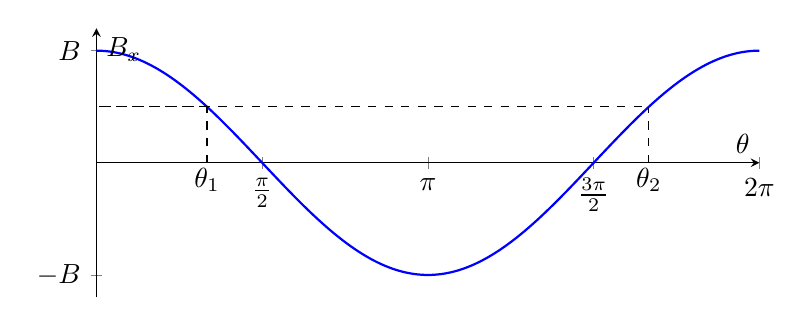
\begin{tikzpicture}
\begin{axis}[
    axis lines=middle,
    xlabel={$\theta$},
    ylabel={$B_x$},
    xmin=0, xmax=2*pi, ymin=-1.2, ymax=1.2,
    xtick={0, 1.5708, 3.1416, 4.7124, 6.2832},
    xticklabels={{$0$}, {$\frac{\pi}{2}$}, {$\pi$}, {$\frac{3\pi}{2}$}, {$2\pi$}},
    ytick={-1, 0, 1},
    yticklabels={{$-B$}, {$0$}, {$B$}},
    width=10cm, height=5cm
]
\addplot [domain=0:6.2832, samples=100, smooth, thick, blue] {cos(deg(x))};

\coordinate (bx_val) at (axis cs:0, 0.5);
\coordinate (theta1) at (axis cs:1.0472, 0);
\coordinate (theta2) at (axis cs:5.2360, 0);

\draw [dashed] (theta1 |- bx_val) -- (bx_val) -- (theta2 |- bx_val);
\draw [dashed] (theta1) -- (theta1 |- bx_val);
\draw [dashed] (theta2) -- (theta2 |- bx_val);

\node at (axis cs:1.0472, -0.15) {$\theta_1$};
\node at (axis cs:5.2360, -0.15) {$\theta_2$};
\node[anchor=east] at (axis cs:-0.3, 0.5) {$B_x$};
\end{axis}
\end{tikzpicture}
\end{center}

For a given value of $B_x$ (where $-B < B_x < B$), there are two angles $\theta_1$ and $\theta_2 = 2\pi - \theta_1$ such that $B_x = B \cos \theta_1 = B \cos \theta_2$. (Let $\theta_1 = \arccos(B_x/B)$).
We use the general formula: $\ProbDens_{B_x}(B_x) = \sum_{i=1,2} \ProbDens_\theta(\theta_i) \left| \deriv{\theta}{B_x} \right|_{\theta=\theta_i}$.
We need the derivative $\deriv{\theta}{B_x}$. It's easier to compute $\deriv{B_x}{\theta}$:
\[ \deriv{B_x}{\theta} = \deriv{}{ \theta} (B \cos \theta) = -B \sin \theta \]
So, $\left| \deriv{\theta}{B_x} \right| = \frac{1}{|-B \sin \theta|} = \frac{1}{B |\sin \theta|}$.
Since $\sin^2\theta + \cos^2\theta = 1$, $|\sin \theta| = \sqrt{1-\cos^2\theta} = \sqrt{1-(B_x/B)^2} = \frac{\sqrt{B^2-B_x^2}}{B}$.
Therefore, $\left| \deriv{\theta}{B_x} \right| = \frac{1}{B (\sqrt{B^2-B_x^2}/B)} = \frac{1}{\sqrt{B^2-B_x^2}}$.
This derivative is the same for $\theta_1$ and $\theta_2$ since $|\sin(\theta_1)| = |\sin(2\pi-\theta_1)|$.

Now apply the formula:
\begin{align*} \ProbDens_{B_x}(B_x) &= \ProbDens_\theta(\theta_1) \left| \deriv{\theta}{B_x} \right|_{\theta_1} + \ProbDens_\theta(\theta_2) \left| \deriv{\theta}{B_x} \right|_{\theta_2} \\ &= \left( \frac{1}{2\pi} \right) \frac{1}{\sqrt{B^2-B_x^2}} + \left( \frac{1}{2\pi} \right) \frac{1}{\sqrt{B^2-B_x^2}} \\ &= 2 \times \frac{1}{2\pi} \frac{1}{\sqrt{B^2-B_x^2}} \end{align*}
\[ \ProbDens_{B_x}(B_x) = \frac{1}{\pi \sqrt{B^2 - B_x^2}} \quad \text{for } -B < B_x < B \]
This distribution is peaked near $B_x = \pm B$ and minimum at $B_x = 0$.

\begin{center}
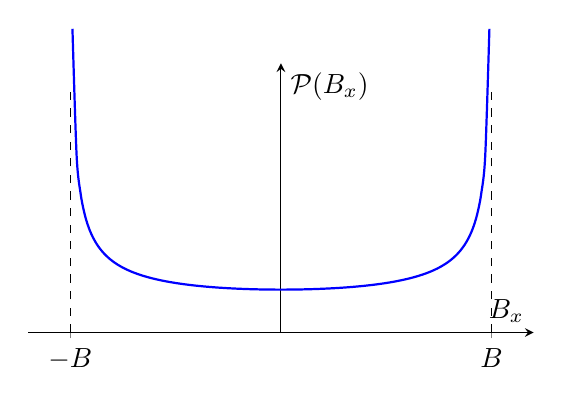
\begin{tikzpicture}
\begin{axis}[
    axis lines=middle,
    xlabel=$B_x$,
    ylabel=$\mathcal{P}(B_x)$,
    xmin=-1.2, xmax=1.2, 
    ymin=0, ymax=2,
    xtick={-1, 0, 1},
    xticklabels={{$-B$}, {$0$}, {$B$}},
    ytick=\empty,
    width=8cm, height=5cm,
    domain=-0.99:0.99, 
    samples=101, 
    clip=false
]
\addplot [smooth, thick, blue] {1/(pi*sqrt(1-x^2))};

% Indicate distribution range
\draw [dashed] (axis cs:-1, 0) -- (axis cs:-1, 1.8);
\draw [dashed] (axis cs:1, 0) -- (axis cs:1, 1.8);
\end{axis}
\end{tikzpicture}
\end{center}


\end{document}
